\documentclass[sigconf,authordraft]{acmart}

\AtBeginDocument{%
  \providecommand\BibTeX{{%
    Bib\TeX}}}

% Draft-friendly ACM settings.
% Replace these metadata fields later when you know the target venue.
\setcopyright{none}
\settopmatter{printacmref=false}
\renewcommand\footnotetextcopyrightpermission[1]{}
\pagestyle{plain}

\acmConference[FMoE Draft]{Draft Venue Placeholder}{2026}{TBD}
\acmBooktitle{Draft Template for FMoE Paper}
\acmDOI{}
\acmISBN{}

% ------------------------------------------------------------------
% Notes for future editing
% ------------------------------------------------------------------
% Figure example:
% \begin{figure}[t]
%   \centering
%   \includegraphics[width=\linewidth]{figures/overview.pdf}
%   \caption{Overall framework of FMoE.}
%   \label{fig:overview}
% \end{figure}
%
% Bibliography example:
% 1) Create refs.bib in the same project folder.
% 2) Add entries there.
% 3) Uncomment the bibliography commands at the end of this file.

\begin{document}

\title[FeaturedMoE for Sequential Recommendation]{FeaturedMoE: Feature-Guided Mixture-of-Experts for Sequential Recommendation}

\author{First Author}
\affiliation{%
  \institution{KAIST}
  \department{Kim Jaechul Graduate School of AI}
  \city{Daejeon}
  \country{Republic of Korea}}
\email{first.author@kaist.ac.kr}

\author{Second Author}
\affiliation{%
  \institution{KAIST}
  \department{Kim Jaechul Graduate School of AI}
  \city{Daejeon}
  \country{Republic of Korea}}
\email{second.author@kaist.ac.kr}

\renewcommand{\shortauthors}{Author et al.}

\begin{abstract}
Mixture-of-experts (MoE) architectures are increasingly adopted in sequential recommendation for their promise of expert specialization, yet routing in many existing models remains largely a black-box function of hidden states. While such hidden-only routing can be effective, the meaning of expert assignment remains implicit, making it difficult to verify whether experts truly capture meaningful behavioral regimes. Meanwhile, feature-aware recommenders typically use side information to enrich sequence representations, leaving the computation path itself unguided. We propose FeaturedMoE (FMoE), a feature-guided modular architecture that bridges these two lines by turning compact behavioral features into explicit routing guidance. Rather than relying on rich dataset-specific metadata, FMoE derives behavioral cues from widely available raw signals in sequential data---namely sessionized interaction order, timestamps, and item categories---and organizes them into complementary feature families that guide macro, mid, and micro routing stages. Extensive experiments show that FMoE does not require a large handcrafted feature bank: compact multi-family feature templates remain effective, stage organization and composition materially affect performance, and corrupted or semantically misaligned cues consistently weaken the model. These findings suggest that common raw signals can be transformed into practical and inspectable routing priors for MoE-based sequential recommendation.
\end{abstract}

% Add proper CCS terms later if needed for the final submission.
% \begin{CCSXML}
% ...
% \end{CCSXML}
% \ccsdesc[500]{...}

\keywords{sequential recommendation, mixture of experts, conditional computation, routing, behavioral features}

\maketitle

\section{Introduction}
Sequential recommendation is commonly formulated as a next-item prediction problem over a user's interaction history. In practice, however, user behavior is rarely governed by a single homogeneous signal. Persistent personal preference, the temporary intent formed within the current session, and short-range transition dynamics often coexist in the same sequence. Strong sequential backbones can model these signals jointly, but they still tend to process them through largely shared computation. As a result, distinct behavioral states are compressed into a single representation space, making it difficult to decide when the model should rely more on long-lived preference, session context, or immediate action patterns.

A common response is to inject additional information. Time-aware recommenders incorporate temporal intervals, long--short preference models separate broad and recent context, and feature-aware recommenders fuse side information into representations or attention layers. These approaches have been highly useful, but they often remain representation-centric: extra signals are added to make hidden states richer, while the computation itself is still mostly shared. Moreover, many side-information methods implicitly assume feature schemas that are not consistently available across datasets. This makes it natural to ask a different question: can a small set of common behavioral cues organize the computation of a sequential recommender, rather than merely decorate its input representation?

\begin{figure}[t]
  \centering
  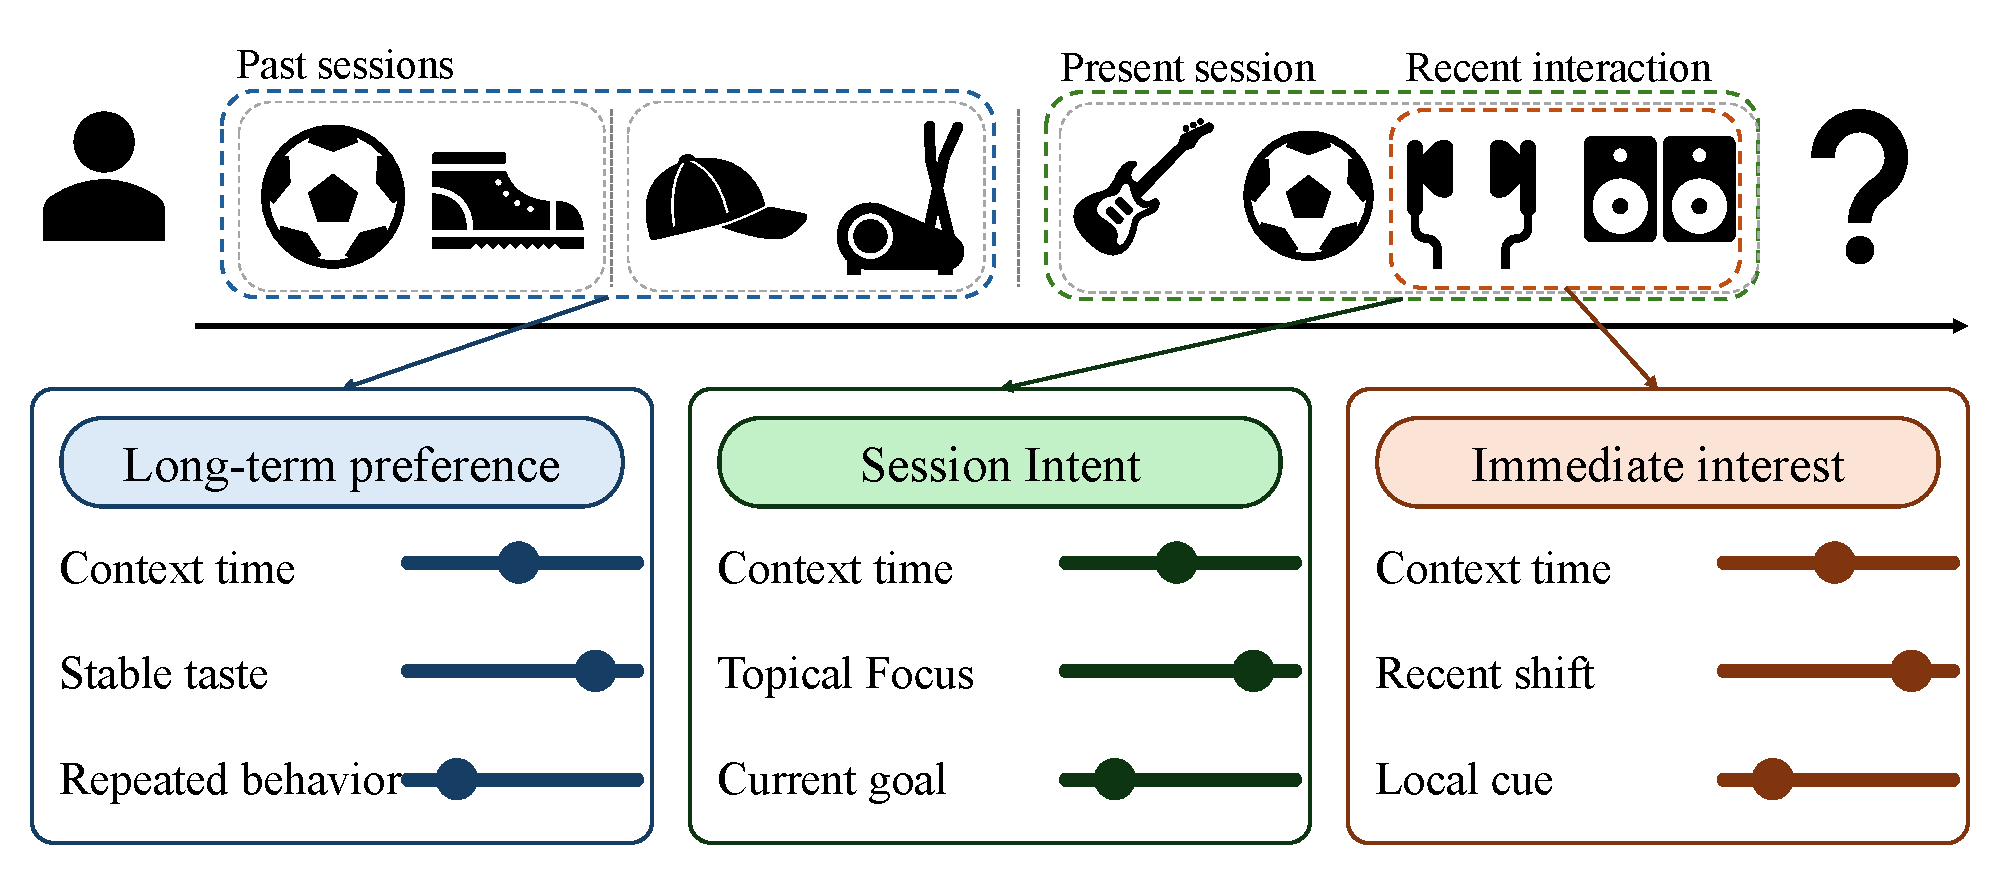
\includegraphics[width=\columnwidth]{figures/figure1_intro_motivation.pdf}
  \caption{Illustrative motivation of FMoE. A single sessionized interaction history can be summarized into compact behavioral features that reflect long-term preference, session intent, and immediate interest.}
  \label{fig:intro-behavioral-features}
\end{figure}

\begin{figure*}[!t]
  \centering
  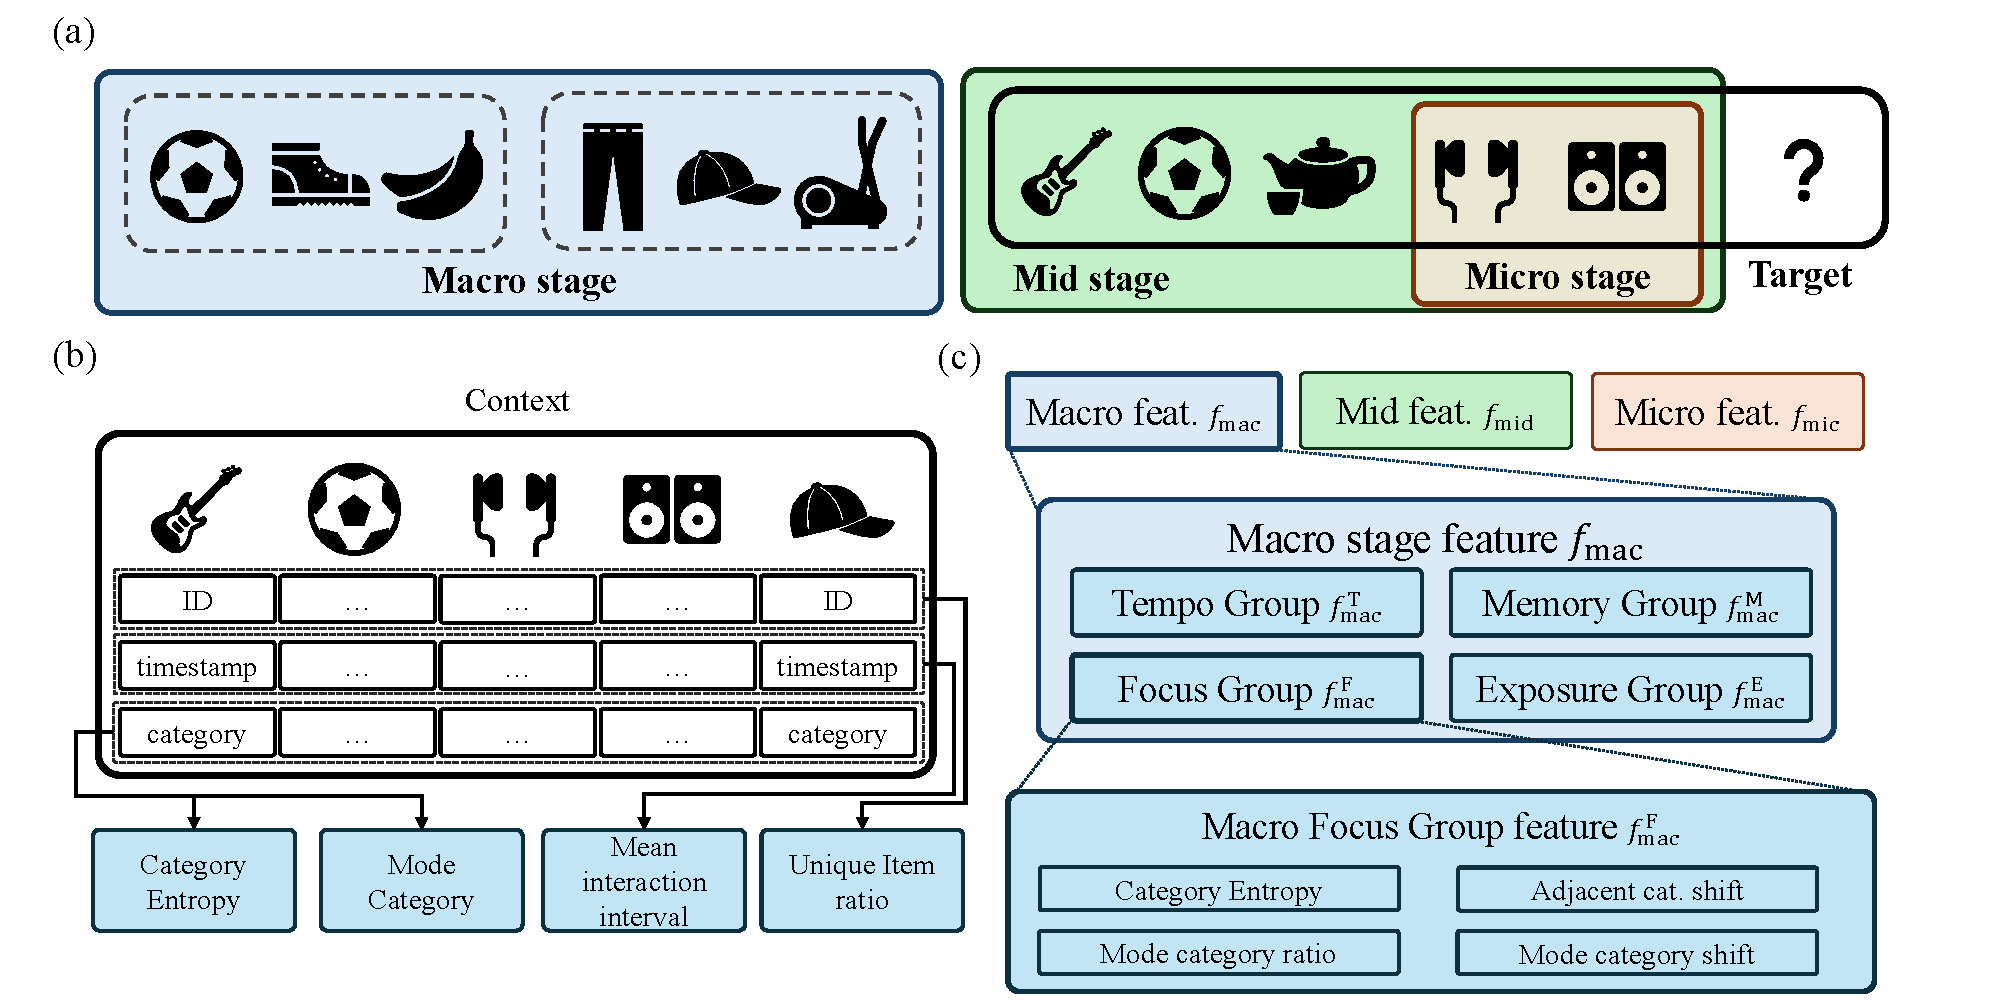
\includegraphics[width=0.94\textwidth]{figures/figure2_feature_construction.pdf}
  \caption{Behavioral feature construction in FMoE. (a) Stage-dependent observation scopes are defined around target position $t$: macro uses preceding sessions, mid uses the current-session prefix, and micro uses the most recent interactions. (b) Common raw signals such as interaction order, timestamps, and categories are converted into lightweight scalar descriptors within each scope. (c) The resulting stage feature is reorganized into shared behavioral groups (Tempo, Focus, Memory, and Exposure), while the scalar values remain stage-specific.}
  \label{fig:feature-construction}
\end{figure*}

We answer this question with FeaturedMoE (FMoE), a feature-guided mixture-of-experts architecture built on a sequential backbone. The key idea is to treat simple behavioral features as routing control signals. Instead of depending on rich metadata, FMoE uses portable cues derived from information that is commonly available in many recommendation datasets, such as sessionized order, timestamps, and item categories. These cues are grouped into behavioral feature families designed to reflect three complementary aspects of user behavior: long-term tendency, session-level context, and local transition tendency. FMoE then uses these families to guide expert routing across macro, mid, and micro stages, so that different behavioral states may trigger different computation paths.

The remainder of this paper is organized as follows. Section~\ref{sec:method} presents the overall FMoE framework and its routing design. Section~\ref{sec:experiments} describes the experimental setup and evaluation plan. Section~\ref{sec:conclusion} concludes the paper.

\section{Related Work}
We briefly review sequential recommendation backbones, feature-aware recommendation, recommendation-oriented mixture-of-experts models, and recent efforts on interpretable or controllable routing. Depending on the target venue and page budget, this discussion can remain as a short standalone section or be folded into the introduction.

\section{Methodology}
\label{sec:method}

\subsection{Problem Definition and Overall Framework}
\label{sec:problem-framework}
Sequential recommendation aims to predict the next item a user will interact with from the user's past behavior sequence. In our setting, the interaction history is organized into sessions, where a session denotes a contiguous period of activity corresponding to a coherent visit or intent. For readability, we omit the user index and describe the history of a single user. Let $\mathcal{S} = [s_1, \dots, s_M]$ denote the session sequence, where the $m$-th session is written as $s_m = [x_1, \dots, x_{|s_m|}]$. Each interaction $x_t$ contains an item ID and timestamp, and each item may additionally be associated with a category label. Given the observed interaction history, the goal is to predict the next item.

FMoE is built on top of a SASRec backbone. We emphasize this point because the backbone itself remains intentionally simple: the input structure is the same as in standard sequential recommendation, and the main architectural change is the introduction of mixture-of-experts computation. The key idea is that expert routing is not determined only from hidden representations. Instead, FMoE constructs compact behavioral features from widely available raw sequential signals, such as sequence order, timestamps, and item categories, and uses them to guide expert selection. In this way, FMoE preserves the strong and simple sequential modeling capability of SASRec while adding an explicit behavioral control signal to the computation path.

Let $\mathbf{h}_t$ denote the hidden state at position $t$, and let $\mathbf{f}_t$ denote the behavioral feature used for routing. The router produces expert weights $\boldsymbol{\pi}_t$, and the hidden representation is transformed by a weighted combination of experts:
\[
\tilde{\mathbf{h}}_t
=
\sum_{e=1}^{E}
\pi_{t,e}\,\mathrm{Expert}_e(\mathbf{h}_t).
\]
FMoE applies this routing mechanism across three behavioral levels---macro, mid, and micro---so that long-term tendency, session-level context, and immediate local transition can guide expert computation at different temporal scales. The following subsections describe how these behavioral features are constructed and how the stage-wise routers are designed.

\begin{figure*}[!t]
  \centering
  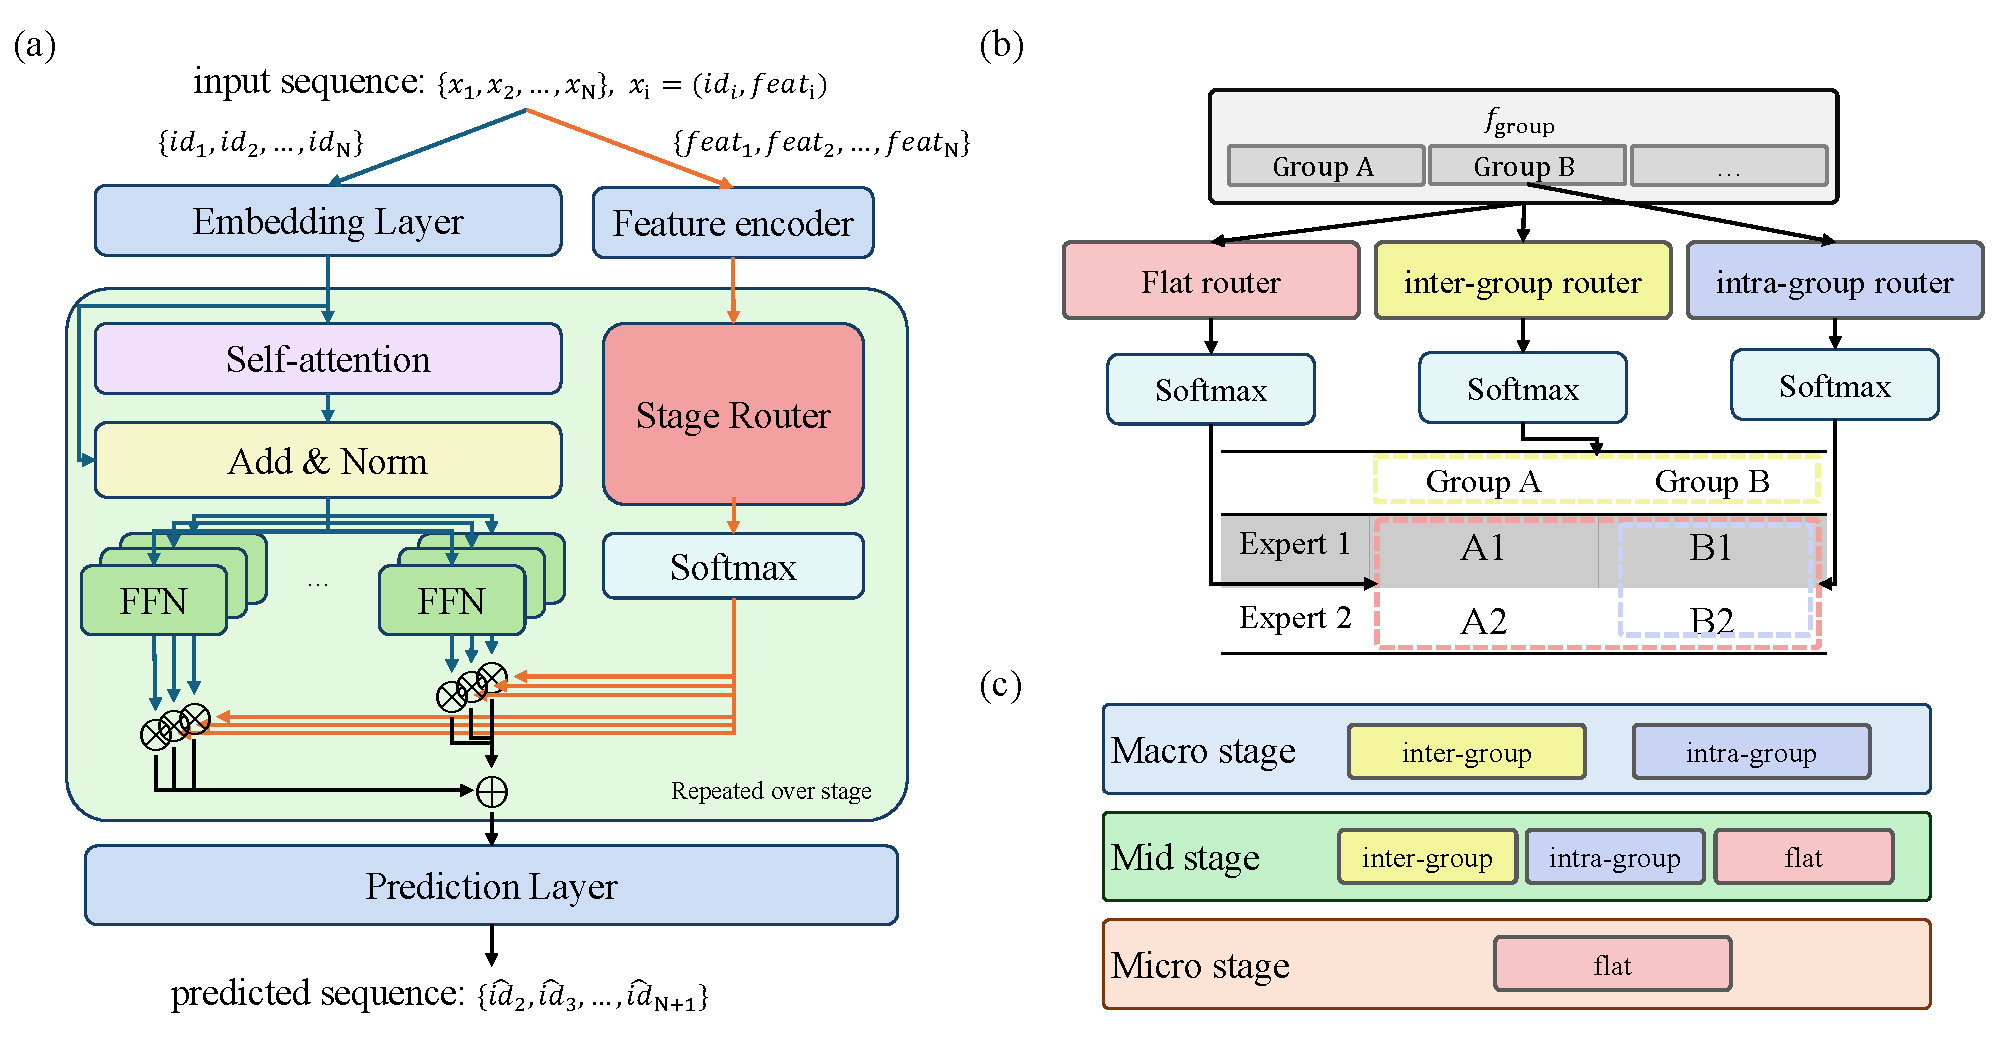
\includegraphics[width=0.94\textwidth]{figures/figure3_framwork.pdf}
  \caption{Feature-guided FMoE routing framework. (a) FMoE keeps the SASRec backbone and replaces shared feed-forward computation with stage-wise mixture-of-experts routing; hidden states flow through expert FFNs, while stage features are used only to compute routing weights. (b) The routing module is decomposed into reusable primitives: \texttt{a\_joint} produces flat expert logits, \texttt{b\_group} produces group logits, and \texttt{d\_cond} produces group-conditional intra-group logits. (c) Different stages use different wrappers: macro uses $\log(b \times d)$, mid uses $\alpha_{\mathrm{struct}}\log(b \times d) + \alpha_a a$, and micro uses $a$ only.}
  \label{fig:framework}
\end{figure*}
\subsection{Behavioral Feature Construction from Raw Sequential Signals}
\label{sec:feature-construction}

Figure~\ref{fig:feature-construction} summarizes the construction pipeline in three steps. Panel~(a) defines the stage-specific observation scopes around the same prediction target, panel~(b) shows how raw sequential metadata are reduced to lightweight scalar descriptors, and panel~(c) shows how those descriptors are grouped into a structured stage feature. The emphasis here is not an exhaustive catalog of handcrafted statistics. Instead, the point is that common raw signals can be turned into a small routing feature bank with clear temporal semantics.

\subsubsection{Raw Signals and Scalar Summaries}

Starting from the notation in Section~\ref{sec:problem-framework}, recall that the current session is written as $s_m = [x_1, \dots, x_{|s_m|}]$. For each interaction $x_t$, FMoE uses only signals that are commonly available in sequential recommendation datasets: item identity $i_t$, timestamp $\tau_t$, and, when available, category label $c_t$. We additionally allow item-level popularity statistics computed from the training corpus. These inputs are deliberately simple. Instead of adding a separate metadata encoder, FMoE converts them into low-dimensional scalar descriptors that can steer routing.

Figure~\ref{fig:feature-construction}(a) shows the three observation scopes defined around the same target position. The macro stage summarizes preceding sessions, the mid stage uses the current-session prefix, and the micro stage focuses on a short recent context immediately before the target. Figure~\ref{fig:feature-construction}(b) then illustrates how raw signals from a given scope are mapped to scalar descriptors, such as interval-, category-, or popularity-related summaries. The descriptor template is shared across stages, but its interpretation depends on the temporal range from which it is extracted.

Formally, let $\mathcal{R}$ denote an observation range and let
\[
\mathcal{A}(\mathcal{R}) = [a_1(\mathcal{R}), \dots, a_K(\mathcal{R})]
\]
be the vector of scalar summaries extracted from that range, where each $a_k(\cdot)$ is a lightweight aggregation such as a count, ratio, mean, entropy, or trend statistic. This notation is intentionally generic: the exact scalar list may vary across datasets, but the construction principle remains the same. FMoE does not assume a rich side-information schema; it reconstructs routing cues from raw sequential evidence that is already present in standard interaction logs.

\subsubsection{Compact Feature Families}

The scalar summaries are not treated as an unstructured list. FMoE groups them into four behavioral families: \textit{Tempo}, \textit{Focus}, \textit{Memory}, and \textit{Exposure}. Tempo captures pace and interval patterns. Focus describes how concentrated behavior is around categories and how often the user switches among them. Memory reflects repetition, recurrence, and overlap with previously observed context. Exposure summarizes the popularity level of consumed items and its local drift.

This grouping step corresponds to Figure~\ref{fig:feature-construction}(c). The semantic group definitions are shared across stages, but the actual scalar values differ because each stage observes a different temporal window. Let $\mathbf{f}$ denote a generic routing feature vector. We write it as
\[
\mathbf{f}
=
[\mathbf{f}^{\mathrm{tempo}} \,\|\, \mathbf{f}^{\mathrm{focus}} \,\|\, \mathbf{f}^{\mathrm{memory}} \,\|\, \mathbf{f}^{\mathrm{exposure}}],
\]
where each block corresponds to one behavioral family. This grouping is mainly semantic rather than architectural: it presents the router with a structured view of behavior instead of a flat collection of unrelated statistics.

\subsubsection{Stage-Specific Feature Views}

The same four feature families are used at all stages, but they are computed over different observation ranges. Figure~\ref{fig:feature-construction}(a) visualizes these scopes around the same target position, while Figure~\ref{fig:feature-construction}(c) shows the shared group layout. With macro history window $H$ ($H=5$ in our main setting), the stage-dependent ranges are
\begin{align}
\mathcal{R}^{\mathrm{macro}} &= [s_{\max(1,m-H)}, \dots, s_{m-1}], \\
\mathcal{R}^{\mathrm{mid}}_t &= [x_1, \dots, x_{t-1}], \\
\mathcal{R}^{\mathrm{micro}}_t &= [x_{\max(1,t-5)}, \dots, x_{t-1}].
\end{align}
Applying the scalar-summary operator $\mathcal{A}(\cdot)$ to these ranges gives
\begin{align}
\mathbf{f}^{\mathrm{macro}} &= \mathcal{A}(\mathcal{R}^{\mathrm{macro}}), \\
\mathbf{f}^{\mathrm{mid}}_t &= \mathcal{A}(\mathcal{R}^{\mathrm{mid}}_t), \\
\mathbf{f}^{\mathrm{micro}}_t &= \mathcal{A}(\mathcal{R}^{\mathrm{micro}}_t).
\end{align}

The macro view is derived from past sessions and remains fixed within the current session. It mainly reflects broad preference and recurring consumption tendency. The mid view is computed from the current-session prefix and is updated at every position $t$, so it tracks evolving session intent. The micro view uses only the most recent interactions before position $t$, making it sensitive to immediate interest and next-step transition cues.

In this way, FMoE combines a shared semantic taxonomy with stage-dependent observation scopes and obtains a compact coarse-to-fine feature bank for routing. The next subsection explains how these stage-specific features are translated into expert weights and why different routing wrappers are assigned to the macro, mid, and micro stages.
\subsection{Feature-Guided Multi-Stage Routing}

Section~\ref{sec:feature-construction} defined compact stage-specific feature views from raw sequential signals. We now explain how these features are translated into routing decisions. Figure~\ref{fig:framework}(a) shows the overall computation flow, Figure~\ref{fig:framework}(b) separates the router into reusable primitives, and Figure~\ref{fig:framework}(c) shows how the three stages compose those primitives differently. Throughout this subsection, we keep the notation light and show stage superscripts only when they are needed.

\subsubsection{Routing Principle and Stage Placement}

FMoE keeps the SASRec encoder as the main hidden-state backbone and replaces shared feed-forward computation with stage-wise mixture-of-experts routing. At position $t$ and stage $s$, the backbone provides hidden state $\mathbf{h}_t$, while the corresponding stage feature $\mathbf{f}^{(s)}_t$ is used only for routing. The stage router first produces expert logits, converts them to routing weights, and then applies a weighted combination of expert FFNs to the hidden state:
\begin{align}
\mathbf{q}^{(s)}_t &= \mathrm{Router}_s(\mathbf{f}^{(s)}_t), \\
\boldsymbol{\pi}^{(s)}_t &= \mathrm{softmax}\!\left(\mathbf{q}^{(s)}_t / \tau_s\right), \\
\tilde{\mathbf{h}}^{(s)}_t &= \sum_{e=1}^{E} \pi^{(s)}_{t,e}\,\mathrm{Expert}^{(s)}_e(\mathbf{h}_t).
\end{align}

This separation is central to FMoE. The feature branch decides which experts should be emphasized, whereas the expert branch transforms only the backbone hidden state. As shown in Figure~\ref{fig:framework}(a), the same principle is used at the macro, mid, and micro stages; what changes across stages is the temporal meaning of the feature and the wrapper used to construct $\mathbf{q}^{(s)}_t$.

\subsubsection{Macro Router: Structured Group-First Routing}

The macro stage is driven by features computed from preceding sessions. As discussed in Section~\ref{sec:feature-construction}, this view is stable within the current session and mainly reflects long-term preference and recurring consumption tendency. In the implementation, the macro stage uses wrapper \texttt{w4\_bxd}, which combines the \texttt{b\_group} and \texttt{d\_cond} primitives.

Let $p_b(g \mid \mathbf{f})$ be the group probability produced by \texttt{b\_group} after softmax, and let $p_d(e \mid g,\mathbf{f})$ be the intra-group expert probability produced by \texttt{d\_cond}. The macro router forms the joint structured probability
\[
J^{\mathrm{macro}}_t(g,e)
=
p_b(g \mid \mathbf{f}^{\mathrm{macro}})\,
p_d(e \mid g, \mathbf{f}^{\mathrm{macro}}),
\]
and then converts it into expert logits in logit space:
\[
\mathbf{q}^{\mathrm{macro}}_t
=
\log J^{\mathrm{macro}}_t.
\]
The final macro routing weights are obtained by
\[
\boldsymbol{\pi}^{\mathrm{macro}}_t
=
\mathrm{softmax}\!\left(\mathbf{q}^{\mathrm{macro}}_t/\tau_{\mathrm{macro}}\right).
\]
This exactly matches the \texttt{w4\_bxd} wrapper in code: the group and intra-group branches are normalized first, their probabilities are multiplied, and the resulting joint probability is mapped back to expert logits by a logarithm. Intuitively, the macro stage first identifies a broad behavioral regime and only then resolves expert preference within that regime.

\subsubsection{Mid Router: Hybrid Group-Aware Routing}

The mid stage uses the current-session prefix and is updated at every position. It is therefore more adaptive than the macro stage, but it still retains meaningful group structure. In the implementation, the mid stage uses wrapper \texttt{w6\_bxd\_plus\_a}, which combines the structured branch from \texttt{b\_group} and \texttt{d\_cond} with the direct flat branch \texttt{a\_joint}.

Using the same structured joint probability as in the macro stage,
\begin{align}
J^{\mathrm{mid}}_t(g,e)
&=
p_b(g \mid \mathbf{f}^{\mathrm{mid}}_t)\,
p_d(e \mid g, \mathbf{f}^{\mathrm{mid}}_t), \\
\mathbf{q}^{\mathrm{struct}}_t
&=
\log J^{\mathrm{mid}}_t,
\end{align}
and letting $\mathbf{q}^{\mathrm{flat}}_t$ denote the flat expert logits from \texttt{a\_joint}, the wrapper forms
\begin{align}
\mathbf{q}^{\mathrm{mid}}_t
&=
\alpha_{\mathrm{struct}} \mathbf{q}^{\mathrm{struct}}_t
+
\alpha_a \mathbf{q}^{\mathrm{flat}}_t,
\\
\boldsymbol{\pi}^{\mathrm{mid}}_t
&=
\mathrm{softmax}\!\left(\mathbf{q}^{\mathrm{mid}}_t / \tau_{\mathrm{mid}}\right).
\end{align}
Unlike the earlier score-product interpretation, the actual code combines the structured and flat branches in logit space. This detail matters: \texttt{w6\_bxd\_plus\_a} first turns the normalized $b \times d$ product into $\log$-space logits and then adds the residual flat logits with coefficients $\alpha_{\mathrm{struct}}$ and $\alpha_a$. The structured path preserves group-aware routing, while the flat path directly corrects expert preference when the current session drifts from the dominant group pattern.

\subsubsection{Micro Router: Direct Expert Routing}

The micro stage focuses on only the most recent interactions before the target position. This feature view is highly local and is intended to capture immediate interest and abrupt next-step-sensitive transitions. In the implementation, the micro stage uses wrapper \texttt{w1\_flat}, which relies only on the flat joint router.

\[
\mathbf{q}^{\mathrm{micro}}_t
=
\mathbf{q}^{\mathrm{flat}}_t,
\qquad
\boldsymbol{\pi}^{\mathrm{micro}}_t
=
\mathrm{softmax}\!\left(\mathbf{q}^{\mathrm{micro}}_t / \tau_{\mathrm{micro}}\right).
\]
This design allows the model to react quickly to short-range transitions without forcing them through an additional group bottleneck. In Figure~\ref{fig:framework}(c), this corresponds to using only the flat primitive.

\subsubsection{Unified Coarse-to-Fine Interpretation}

Taken together, the three routers form a coarse-to-fine hierarchy. The macro stage uses only the structured branch because long-horizon evidence is stable but coarse. The mid stage blends structured and flat branches because session-level intent is organized but still drifting. The micro stage uses only the flat branch because immediate evidence is already sharp enough for fine-grained expert discrimination. The stages therefore differ not only in temporal scope but also in the routing bias assigned to that scope.

\subsection{Training Objective and Router Stabilization}

FMoE is trained with the standard next-item prediction loss together with two router-side stabilizers. In the A6 setting used in our main experiments, the active auxiliary terms are route consistency and z-loss, while optional balance- or bias-related regularizers are disabled. The goal is to keep feature-guided routing behaviorally coherent and numerically stable without changing the base recommendation objective.

\subsubsection{Main Recommendation Objective}

Let $\mathbf{z}$ denote the final prediction logits for the sequence and let $y$ be the target next item. The main loss is the standard cross-entropy objective
\[
\mathcal{L}_{\mathrm{CE}}
=
-\log \frac{\exp z_y}{\sum_{j}\exp z_j}.
\]
FMoE does not change the prediction target itself. It changes the computation path used to produce that prediction by making expert selection depend on behavioral features.

\subsubsection{Route Consistency Regularization}

A key motivation of FMoE is that routing should respond to behavioral features rather than emerge only implicitly from hidden states. If two samples are very similar in raw behavioral feature space, their routing patterns should also be close. The route consistency loss encourages this property.

In the implementation, we first summarize each sample by averaging its raw feature tensor over the sequence dimension. Let
\[
\bar{\mathbf{u}}_i
=
\frac{1}{L_i}\sum_{t=1}^{L_i}\mathbf{u}_{i,t}
\]
be the pooled raw feature vector for sample $i$, where $L_i$ is the valid sequence length. We normalize these vectors, compute pairwise cosine similarity within the mini-batch, select a small set of nearest neighbors for each sample, and keep only pairs above a similarity threshold $\gamma$. This gives a set $\mathcal{P}$ of reliable neighbor pairs in feature space.

For routing comparison, we aggregate token-level routing weights into a session-level routing distribution. For stage $s \in \mathcal{T}$, let
\[
\bar{\boldsymbol{\pi}}_i^{(s)}
=
\frac{1}{L_i}\sum_{t=1}^{L_i}\boldsymbol{\pi}^{(s)}_{i,t}
\]
denote the mean routing distribution of sample $i$ over valid positions at stage $s$. The consistency loss is then
\[
\mathcal{L}_{\mathrm{cons}}
=
\frac{1}{|\mathcal{T}|}
\sum_{s \in \mathcal{T}}
\frac{1}{|\mathcal{P}|}
\sum_{(i,j)\in \mathcal{P}}
\mathrm{JSD}\!\left(\bar{\boldsymbol{\pi}}_i^{(s)}, \bar{\boldsymbol{\pi}}_j^{(s)}\right),
\]
where $\mathcal{T}=\{\mathrm{macro},\mathrm{mid},\mathrm{micro}\}$ is the set of routing stages. This regularizer does not force a single global routing pattern. It acts only on sufficiently similar feature states, encouraging stage-wise routing to remain semantically stable when the underlying behavioral evidence is nearly the same.

\subsubsection{z-Loss for Router Logit Stabilization}

While route consistency regularizes the semantic behavior of routing, z-loss regularizes its numerical behavior. Since routing weights are produced from pre-softmax expert logits, excessive logit magnitude can make gating overly sharp and unstable.

Following the implementation, we compute a masked average of the squared log-partition value of the router logits at valid positions. Let $\mathbf{q}^{(s)}_{i,t}$ denote the router logits for sample $i$, position $t$, and stage $s$. The z-loss is
\[
\mathcal{L}_{z}
=
\frac{1}{|\mathcal{T}|}
\sum_{s \in \mathcal{T}}
\frac{1}{N_s}
\sum_{(i,t)\in\mathcal{V}_s}
\left(
\log \sum_{e=1}^{E}\exp q_{i,t,e}^{(s)}
\right)^2,
\]
where $\mathcal{V}_s$ is the set of valid positions for stage $s$ and $N_s = |\mathcal{V}_s|$. This term penalizes excessive logit scale and helps keep routing well behaved during training.

\subsubsection{Final Objective}

The final objective is the sum of the recommendation loss and the two routing-side regularizers:
\[
\mathcal{L}
=
\mathcal{L}_{\mathrm{CE}}
+
\lambda_{\mathrm{cons}}\,\mathcal{L}_{\mathrm{cons}}
+
\lambda_{z}\,\mathcal{L}_{z},
\]
where $\lambda_{\mathrm{cons}}$ and $\lambda_z$ control the strength of route consistency and z-loss, respectively. In the A6 setting, this CE-plus-stabilization objective is the full training criterion because the other optional auxiliary terms are turned off.
\section{Experiments}
\label{sec:experiments}

\subsection{Experimental Setup}
This subsection will describe datasets, preprocessing, evaluation metrics, baselines, and implementation details. It is usually enough to keep the main paper concise and move dataset-specific preprocessing details to an appendix if the venue has a strict page limit.

\subsection{Main Results}
This subsection will report the overall comparison against baseline sequential recommenders and MoE-based variants. A table comparing HR@K and NDCG@K or MRR@K across datasets will likely be the main result table.

\subsection{Ablation and Diagnostic Analysis}
This subsection can be used for router design ablations, feature-family ablations, stage composition studies, corrupted-feature sanity checks, and any analysis of routing behavior or expert specialization.

\section{Conclusion}
\label{sec:conclusion}
In this draft, the paper is organized around the claim that compact behavioral cues can serve as explicit routing guidance for mixture-of-experts sequential recommendation. The final conclusion can briefly restate this perspective, summarize the empirical findings, and discuss portability, interpretability, and future extensions of the framework.

% Uncomment after creating refs.bib.
% \bibliographystyle{ACM-Reference-Format}
% \bibliography{refs}

\end{document}
